\subsection{Space Density Evolution}
\label{Sec: Class Density}

In this section, we inspect the evolution of different luminosity classes by visualising the number density of each luminosity bin across redshift (figure \ref{Fig: Class Evo}). By incorporating the class density evolution into our analysis, a better picture of the evolution of galaxies and the co-evolution of AGN can be ascertained. When possible, the $\phi$ values are taken from the existing luminosity bins\footnote{$\phi$ values ending in X.875 and X.375 $\log_{10}(L_{\odot})$ are skipped. Shown bins are 0.25 $\log_{10}(L_{\odot})$ wide.}. Otherwise, $\phi$ values are calculated from the best-fitting LF. The class density evolution (figure \ref{Fig: Class Evo}) can be thought of as the transpose of the LF (figures \ref{Fig: Bolometric IR LF} and \ref{Fig: LF Filled}). The LF and class density are complementary because they allow us to view the number density as an evolution with luminosity and redshift, respectively. 

\begin{figure*}[ht!]
    \centering
    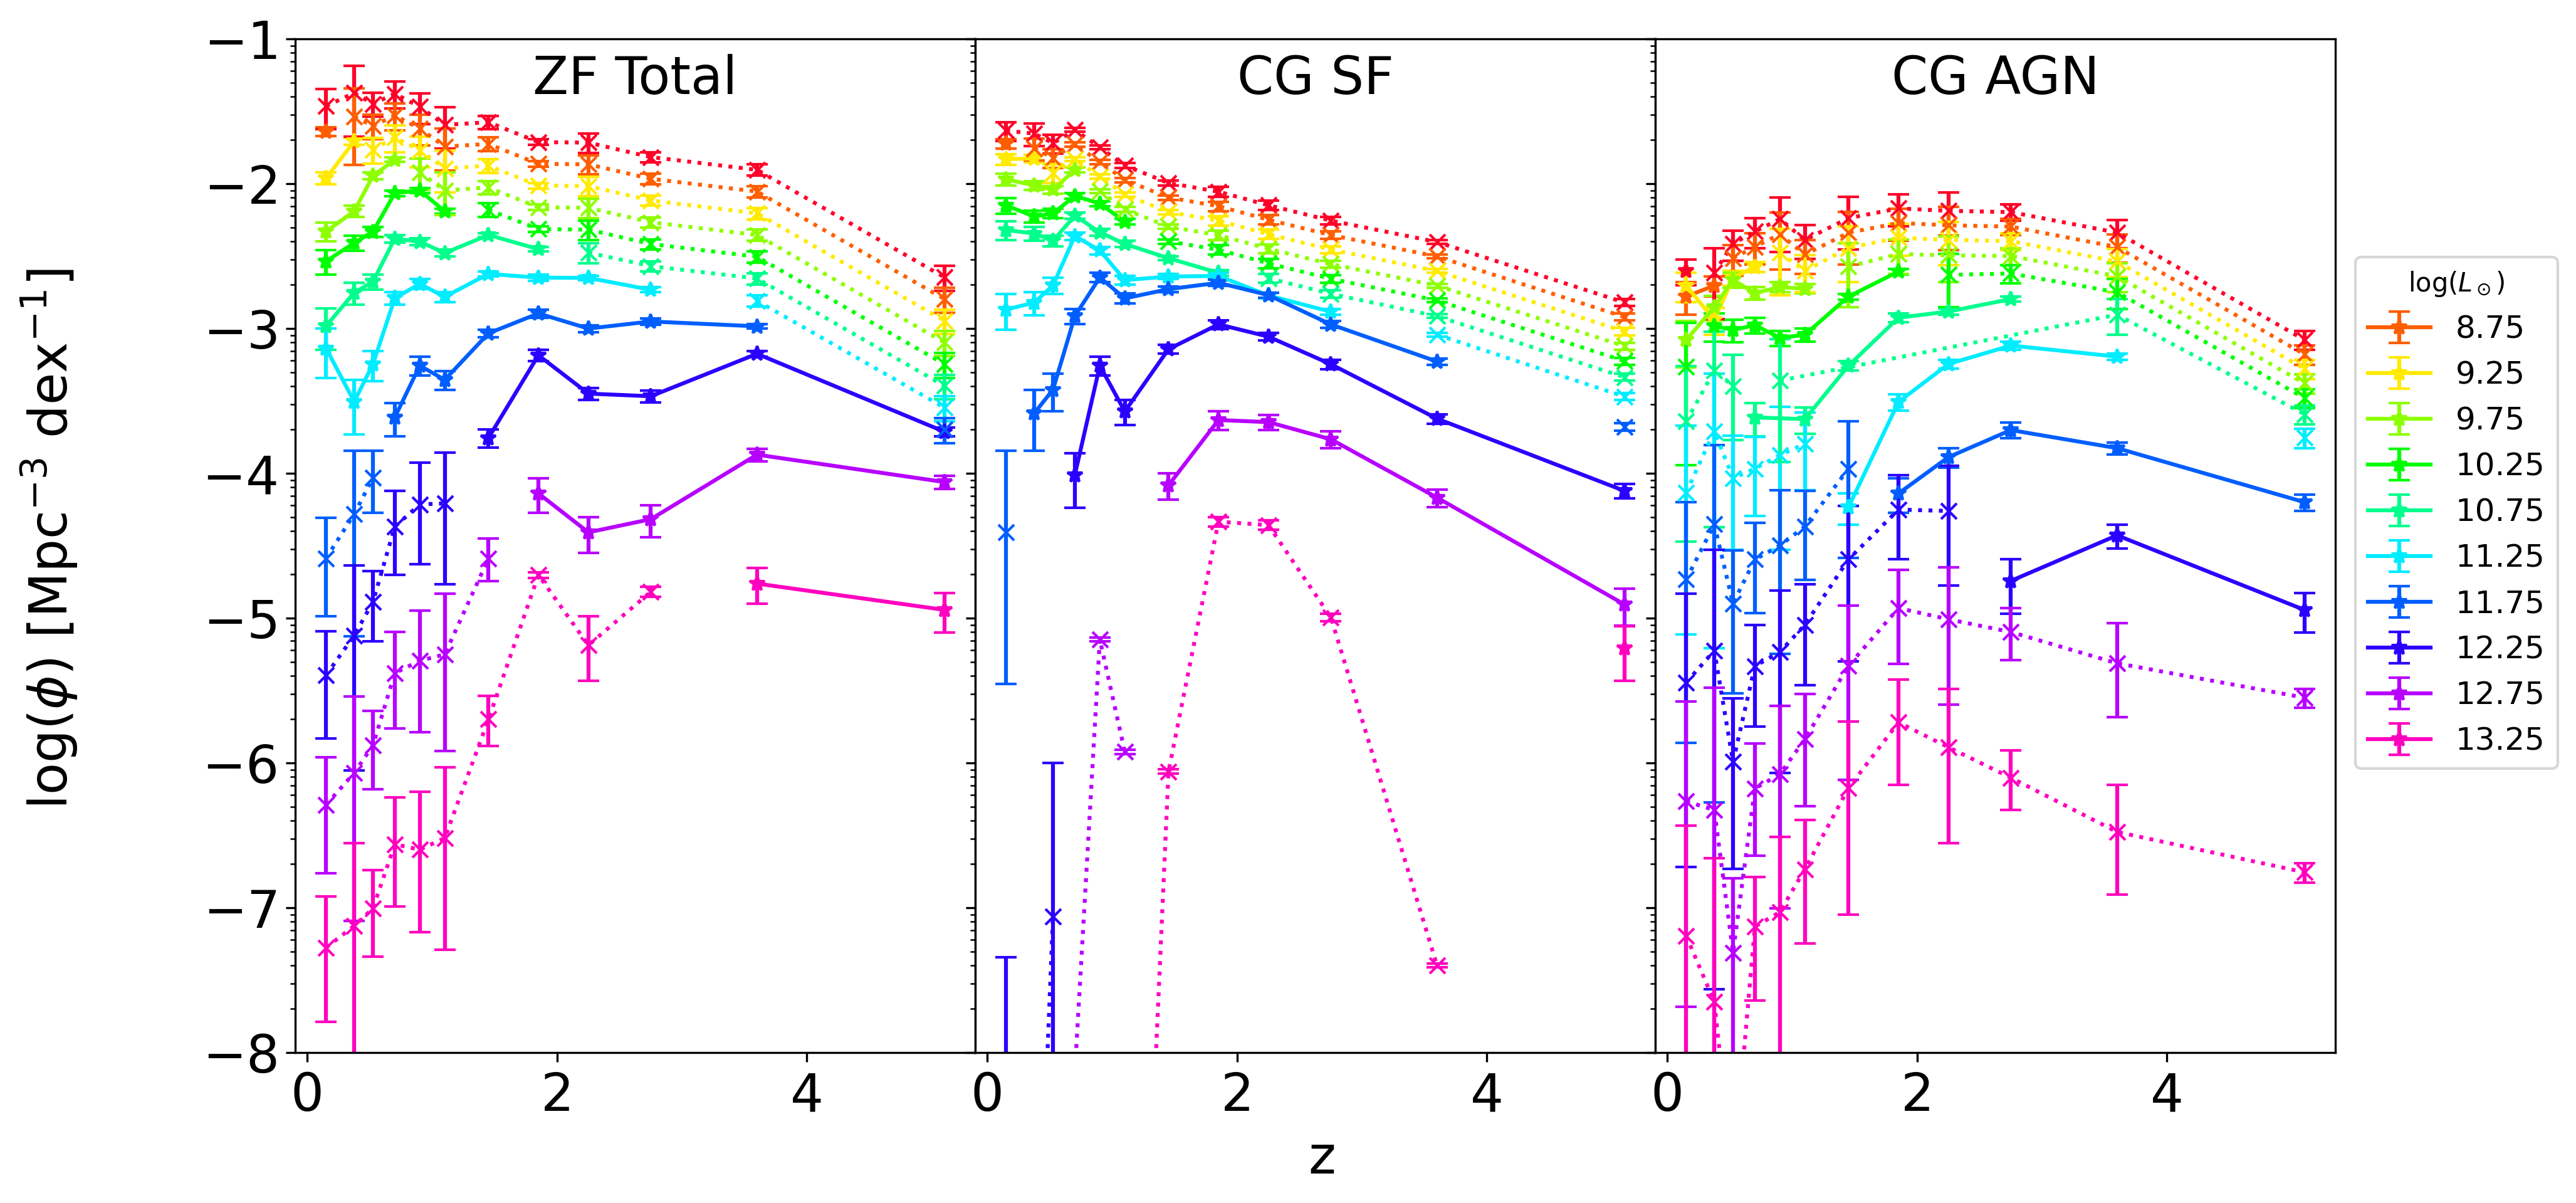
\includegraphics[width=\textwidth]{Figures/Class_Evo.png}
    \caption{Luminosity class evolution as a function of redshift. $\phi$ values connected by straight lines correspond to real values in Figure \ref{Fig: Bolometric IR LF}. $\phi$ values connected by dashed lines are estimated from the best fitting LF. Error bars represent the propagated uncertainty derived from the LF. Real luminosity classes are 0.25 log$(L_{\odot})$ in width and centred in the middle (e.g. 8.5 --- 8.75 is centred on 8.625). Estimated classes are calculated at the centre of the luminosity bin (e.g. 8.625). Not all luminosity bins from Figure \ref{Fig: Bolometric IR LF} are displayed to reduce clutter.}
    \label{Fig: Class Evo}
\end{figure*}

In Figure \ref{Fig: Class Evo}, we present IR luminosity classes as low as $L_{IR}=10^{8.5}\ L_{\odot}$. We find that the space density of ZFOURGE LIRGs and ULIRGs have been consistently declining since at least $z=2$, and likely even earlier for ULIRGs. Galaxies fainter than LIRGs (FIRGs, $L_{IR} < 10^{11} L_{\odot}$) evolve differently, beginning to decline at a lower redshift than their brighter luminosity counterparts. The redshift at which galaxies begin declining in number density is related to their luminosity. ZFOURGE galaxies fainter than $L_{IR} < 10^{9}\ L_{\odot}$ appear to be increasing in number density across all of cosmic time and have yet to begin declining. We find similar agreement in the literature with \cite{rodighiero_mid-_2010} and \cite{gruppioni_herschel_2013} with our results mostly in agreement. We attribute the differences to slight variations in the classes and methods within. FIRGs dominate the ZFOURGE LD from $0<z<1.2$, declining from 74\% to 47\%. LIRGs dominate from $1.2<z<3$, remaining steady with 43\% to 51\% contribution. At $z>3$, ULIRGs dominate LD, increasing rapidly from 38\% to 74\%. In the highest redshift bin, FIRG contribution drops to 5\%

CIGALE SF galaxies evolve differently from ZFOURGE, although similar contributions to the LD are seen. FIRGs dominate LD density from $0<z<1.0$, remaining roughly constant between 49\% to 63\%. LIRGs only dominate LD from $1.0<z<1.2$ with 45\% contribution. ULIRGs dominate LD from $z>1.2$ onwards, with contribution increasing from 48\% to 75\%. Figure \ref{Fig: Class Evo} shows that SF LIRGs evolve similarly to FIRGs at $z>2$. However, the estimated $\phi$ values show an increasing number density with decreasing luminosity for all FIRGs. A possible evolution scenario is theorised for SF: all evolve similarly from high redshift to $z \approx 2$, increasing in number density from high redshift. At and below $z \approx 2$, the brightest FIRG number densities begin to peak and decline earlier than fainter FIRG counterparts, which have yet to start declining. LIRGs decline faster and earlier than FIRGs, and ULIRGs decline faster and sooner than LIRGs. This reflects a \textit{downsizing} scenario in which brighter galaxies peak in number density at higher redshift \citep{merloni_synthesis_2008, wylezalek_galaxy_2014, fiore_agn_2017}.

CIGALE AGN again evolve differently. Faint IR AGN dominate LD from $0 \leq z < 1.7$ and luminous IR AGN dominate LD from $z>1.2$ onwards. Ultra-luminous IR AGN never dominates. The difference between FIRGs and LIRGs is stark. There is a clear, systematic shift in the peak number density with luminosity class. The \textit{downsizing} seen in SF galaxies is more pronounced in AGN. As AGN luminosity increases, the number density of AGN peaks at higher redshifts and declines earlier than their fainter luminosity counterparts. When comparing the \textit{downsizing} effect between SFGs and AGN, it is unmistakable that galaxies with a luminous AGN decline faster and earlier than equally bright SFG counterparts.